%
% exemplo de artigo usando o modelo RITA.cls
%
\documentclass{RITA}
%\usepackage[brazilian]{babel}
\usepackage{graphicx}
\usepackage[utf8]{inputenc}

%
% pre�mbulo
%
\title{Combining artificial intelligence, ontology, and frequency-based approaches to recommend activities in scientific workflows}
\author{
Adilson Lopes Khouri
\footnote{Escola de Artes Ciencias e Humanidades, EACH\\
  \texttt{\{adilson.khouri.usp@gmail.com, luciano.digiampietri@gmail.com\}}}
\and
Luciano Antonio Digiampietri
\footnotemark[1]
}
\RITAvolume{VIII}
\RITAnumber{1}
\RITAyear{2017}

\begin{document}
\maketitle

\begin{abstractinenglish}
The number of activities provided by scientific workflow management systems is large, which requires scientists to know many of them to take advantage of the reusability of these systems. To minimize this problem, the literature presents some techniques to recommend activities during the scientific workflow construction. In this paper we specified and developed a hybrid activity recommendation system considering information on frequency, input and outputs of activities and ontological annotations. Additionally, this paper presents a modeling of activities recommendation as a classification problem, tested using \(5\) classifiers; \(5\) regressors; and a composite approach which uses a Support Vector Machine (SVM) classifier, combining the results of other classifiers and regressors to recommend; and Rotation Forest, an ensemble of classifiers. The proposed technique was compared to related techniques and to classifiers and regressors, using \(10\)-fold-cross-validation, achieving a Mean Reciprocal Rank (MRR) at least \(70\%\) greater than those obtained by classical techniques.
\end{abstractinenglish}

\section{Introduction}
The number of research projects using intensive computing has been growing in areas such as biology, physics, and astronomy. One of the tools to assist in the management and construction of intensive computing experiments are the workflows management systems. \emph{Scientific Workflows} represent structured and ordered processes, constructed manually, semi-automatically or automatically to solve scientific problems using activities, which can be: i) source code blocks; (ii) services; or iii) finished workflows~(\cite{Wang2010}). These systems facilitate the creation of new experiments, sharing of results and reuse of existing activities. Workflows are models to represent a flows of interrelated activities which execution leads to a goal. In this paper the term \emph{workflow} is used as a synonymous of \emph{scientific workflow}.


%There are business workflow wich are sequence of tasks. Tipicaly this kind of workflow have diferent flows and dont use intensive computacional ressources, they are \emph{control flow} oriented instead of \emph{data flow} oriented like scientific workflows. The focus of the paper are scientific workflows.

There is also another type of workflows, the business workflows, whose area of study is known as Business Process Management (BPM). Considering business workflows, the process mining aims to discover, monitor or improve process based on event logs~\cite{Aalst2011}. 

Typically, scientific workflows have an intensive use of computational resources and are \emph{data flow} oriented. On the other hand, business workflows are, typically, \emph{control flow} oriented. In this paper, we focus only on scientific workflows..

Nowadays, there are a large number of activities available in repositories such as \emph{myExperiment}\footnote{http://www.myexperiment.org/} which stores more than $2,500$ workflows and \emph{BioCatalogue}\footnote{https://www.biocatalogue.org/}, which provides more than $2,464$ services. The large number of activities and the low reuse of some activities and workflows motivate the construction of techniques to recommend activities to the scientists during the composition of workflows (\cite{Wang2010}).

In the workflow management systems, activities are typically represented as graphical icons with drag and drop functionality. Thus, it is possible to construct computational experiments by dragging icons and filling in input parameters. Most of these systems provide sets of basic activities that can be used in different domains, for example, an activity that calculates the average value of a dataset is applicable in biology, physics, astronomy, and other areas. However, there is a precondition for reusing and/or creating workflows (without the aid of a recommender system): knowing a great number of available activities to avoid recreate them.

In order to minimize the problem of knowing a large number of activities, several techniques were proposed to recommend activities or to compose workflows. In the first case, which aims to serve an expert user in these systems, during the construction of the workflow, activities are recommended to help to complete the workflow. In the second case, whose goal is to serve a less expert user, several workflows are built, automatically by a computer program combining the input and output of activities, and the user should select which one most satisfies him/her need. In the literature this second process is called: \emph{workflow composition} \cite{Fei2012}.

%The main goal of this paper is to help expert users to reuse activities while they are constructing scientific workflows. This goal will help biologists to construct faster workflows because they wont need to recreate the activities. Additional, this work will prevent the creation of unnecessary activities, the ones you didn’t create because was a similar one in the database.

Although there are already some approaches for recommending activities in workflows, in general, all have some limitations. For example, many of the approaches require a very large data set to enable a frequency based or a machine learning approach. Thus, they do not deal well with sparse data (i.e., the existence of a large set of activities each one of them used only in few workflows). Other solutions need detailed information about authors, workflows, and activities that typically are not available in public repositories of activities and workflows.

This paper presents a hybrid approach for recommending activities in scientific workflows based on the frequency of activities combined with the use of semantics, considering datasets with no provenance information, and without reliability information about the authors of the services and workflows. We also propose a modeling of the problem of recommending activities in scientific workflows to be used by classifiers such as: Support Vector Machine (SVM), Naive Bayes (NB), K-Nearest-Neighbor (KNN), Classification and Regression Trees (CART), and Neural Network (MLP). The following regressors were also used: Support Vector Regression (SVR), CART, Neural Network, Multivariate Adaptive Regression Splines (MARS) and Binomial Regression (BR).

In the section \emph{Relate Work} describes the techniques proposed in the related literature. In the section \emph{Materials and Methods} presents the data source, selected sample, and the modeling of the problem as a classification problem. In the section \emph{Proposed Solutions} describes the proposed solution: our algorithm that combines different characteristics in the recommendation and the recommendation of activities modeled as an artificial intelligence classification problem. In section \emph{Results} we present and discuss a performance comparison of our approach and the approaches from the related literature is presented. In the section \emph{Conclusion} the final considerations are presented.

\section{Related Work}
The related literature presents several techniques to recommend activities in scientific workflows. They will be briefly described in this section, for a complete systematic review we suggest the work of Khouri and Digiampietri, 2015\nocite{Khouri2015}. The works of \cite{Shao2007} and \cite{Shao2009}, which consider the sequential mining of activities as \emph{itemsets}, ignore the order of activities and their semantics. The proposal of \cite{TostaBraganholo2015} disregards only the semantics of activities. The present approach considers the order of activities as an important factor in the recommendation because in data flows applications (such as in scientific workflows) the results depends on the order of the activities. Previous activity could be used to predict the next activity when there is a high frequency of both in the same order. Previous activity could be used to predict the next activity when there is a high frequency of both in the same order.

The work of \cite{Koop2008, Oliveira2008, Wang2009, Zhang2009, Tan2011, Cao2012, Diamantini2012} and \cite{Garijo2013, Yeo2013} consider the order of activities, input, output and data provenance. Their limitations are the need of provenance data, since not all Scientific Workflow Management System (SWMS) stores this information. Besides, they do not use semantic information of workflows and activities. Our approach does not require provenance information and considers the semantics of the information using an ontology.

The work of \cite{Bomfim2005} uses only a mapping between activities and ontology, disregarding the input and output, which potentially generates inefficient recommendations. In our approach, the inputs and outputs of each activity are considered, in addition to the use of a domain ontology. The match between input and output is important to ensure that the output data type of an activity are syntactically compatible with the input of another.

Wang et al, 2008\nocite{Wang2008} and Leng et al, 2010\nocite{Leng2010} use only the posteriori probability of occurrence of a new activity. For example, if there was a workflow where a service \emph{b} call service \emph{c} and \emph{c} call service \emph{d}, during the construction of a new workflow, if the user added the service \emph{b} the system will suggest \emph{c} and \emph{d}. The authors do not consider the use of semantics or even the order of pairs of services (or activities).

The work of \cite{Yao2012} requires calculating the confidence of users and of their workflows. Repositories like \emph{myExperiment} do not require users to fill in this data, thus much of the information related to this aspect is not filled by users. In addition, the authors disregard the semantics of activities and workflows.

The works of \cite{Telea1999, Oliveir2010} and \cite{Zhang2011} disregard the use of semantics to recommend, which is a limitation as discussed by \cite{CorchoGarijo2014, Soomro2015}. In our approach, the frequency is considered in conjunction with the domain ontology.

The works of \cite{CorchoGarijo2014} and \cite{Soomro2015} consider the use of frequency and ontology, as in this approach, but they recommend \emph{subworkflows} which limits the recommendations of activities. Only activities used in common fragments of workflows may be recommended. In other words, if the activity is in the ``middle'' of a \emph{subworkflow} it will never be recommended individually. In our approach, all activities can be recommended even at the end of the recommendation list. In addition, it presents a more comprehensive recommendation, as it deals with activities, \emph{subworkflows} (more than one activity working together as one workflow inside another workflow) and \emph{shims} (data type converters and/or adapters).

\section{Materials and Methods} \label{mat_met}
The workflows were obtained from the \emph{myExperiment} repository, using the program \emph{wget}\footnote{https://www.gnu.org/software/wget/}. After downloading the $2,481$ workflows in \emph{xml} format, the \emph{BeautifulSoup}\footnote{https://www.crummy.com/software/BeautifulSoup/bs4/doc/} code analyzer was used to organize the dataset in a relational database

The data is exported to a simple matrix used for techniques that do not use the order of the activities. And also in an array adapted to modelling the recommendation problem as artificial intelligence binary classification and regression problems. These representation will be described in the following sections.

\subsection{Simple matrix}
The $2481$ contains 73 bioinformatic's workflows related to genome assembly and annotation. These workflows were used in the study case for this paper and they are composed of 280 activities. The activities were converted into a matrix $M_{i, j}$. In this matrix, each line corresponds to a workflow and each column to an activity. $M_{i, j} = 1$ means that the workflow \emph{i} contains the activity \emph{j}. Otherwise, $M_{i, j} = 0$ means that the workflow \emph{i} does not contain the activity \emph{j}. Table~\ref{tabela_matriz_de_dados} presents an fictitious example of a matrix \(M\). To perform the evaluation of the approach, an activity is removed from each row of Table~\ref{tabela_matriz_de_dados}, and a list of possible activities is recommended. The goal of the recommendation system is to correctly identify which activity is missing in the workflow (i.e., the one that was removed).
\begin{table}[htb]
	\begin{center}
	\label{tabela_matriz_de_dados}
	\caption{Input matrix example.}
	\begin{tabular}{ccccc}  \hline
		\textbf{Workflow} & \textbf{Activ\(\mathbf{01}\)} & \textbf{Activ\(\mathbf{02}\)} & \textbf{\(\mathbf{\ldots}\)} & \textbf{Activ\(\mathbf{280}\)}  \\ \hline
		01 			  & 1 			  & 0 			  & \(\ldots\) 	  & 0  				\\ 
		02 			  & 1 			  & 1 			  & \(\ldots\) 	  & 1  				\\ 
		03 			  & 1 			  & 0 			  & \(\ldots\) 	  & 1  				\\ 
		\(\vdots\) 		  			  & \(\vdots\) 	  & \(\vdots\) 	  & \(\vdots\) 	  & \(\vdots\) 		\\ 
		73 			  & 1 			  & 0 			  & \(\ldots\) 	  & 0  				\\ \hline
	\end{tabular}
	\end{center}
\end{table}

\subsection{Adapted Array}
In order to use classification and regression techniques, some changes were proposed in the original dataset (exemplified in Table~\ref{tabela_matriz_de_dados}), which can be viewed in the table~\ref{tabela_matriz_de_dados_adapatada_classificacao_regressao}. Each workflow was replicated \(118\) times. 59 of these correspond to identical copies of the original workflow, while in the other \(59\), one activity was removed from the original workflow and a new activity was added representing a possible recommendation. Thus, for each original workflow, there will be \(59\) correct instances and \(59\) incorrect instances and this type of information will be used to train the classifiers or regressors.
\begin{table}[!htb]
	\begin{center}
	\caption{Input matrix used by classifiers and regressors}
	\label{tabela_matriz_de_dados_adapatada_classificacao_regressao}
	\begin{tabular}{cccccccc}  \hline
		\textbf{\(\#\)} & \textbf{WF} & \textbf{Act\(\mathbf{01}\)} & \textbf{Act\(\mathbf{02}\)} & \textbf{\(\mathbf{\ldots}\)}  &  \textbf{Act\(\mathbf{280}\)} & \textbf{Class} \\ \hline
		1                 & 01            & 1                               & 0                               & \(\ldots\)                       & 0                                & T                \\ 
		2                 & 01            & 1                               & 0                               & \(\ldots\)                       & 0                                & T                \\ 
		\(\vdots\)        & \(\vdots\)    & \(\vdots\)                      & \(\vdots\)                      & \(\vdots\)                       & \(\vdots\)                       & \(\vdots\)       \\ 
		59                & 01            & 1                               & 0                               & \(\ldots\)                       & 0                                & T                \\ 
		1                 & 01            & 0 (removed)                     & 1 (added)                       & \(\ldots\)                       & 0                                & F                \\ 
		2                 & 01            & 0 (removed)                     & 0                               & \(\ldots\)                       & 0                                & F                \\ 
		\(\vdots\)        & \(\vdots\)    & \(\vdots\)                      & \(\vdots\)                      & \(\vdots\)                       & \(\vdots\)                       & \(\vdots\)       \\ 
		59                & 01            & 0 (removed)                     & 0                               & \(\ldots\)                       & 1 (added)                        & F                \\ 
		& \(\vdots\)    &                                 &                                 &                                  &                                  &                  \\ 
		1                 & 73            & 1                               & 1                               & \(\ldots\)                       & 0                                & T                \\ 
		2                 & 73            & 1                               & 1                               & \(\ldots\)                       & 0                                & T                \\ 
		\(\vdots\)        & \(\vdots\)    & \(\vdots\)                      & \(\vdots\)                      & \(\vdots\)                       & \(\vdots\)                       & \(\vdots\)       \\ 
		59                & 73            & 1                               & 1                               & \(\ldots\)                       & 0                                & T                \\ 
		1                 & 73            & 1 (added)                       & 0 (removed)                     & \(\ldots\)                       & 0                                & F                \\ 
		2                 & 73            & 1                               & 0 (removed)                     & \(\ldots\)                       & 0                                & F                \\ 
		\(\vdots\)        & \(\vdots\)    & \(\vdots\)                      & \(\vdots\)                      & \(\vdots\)                       & \(\vdots\)                       & \(\vdots\)       \\ 
		59                & 73            & 1                               & 0 (removed)                     & \(\ldots\)                       & 1 (added)                        & F                \\ \hline
	\end{tabular}
	\end{center}
\end{table}
The choice of \(59\) activities to be recommended was made for two reasons. The first is to select the 59 activities most frequently used in the database. The second is the computational limitation: replicating the \(280\) possible recommendations might be impractical in terms of training. Thus, the number 59 was chosen empirically after some exploratory tests. We have replicated \(59\) instances of identical workflows considered correct, i.e. with the correct activity not removed, to ensure inter-class balancing. The last change was to add a column indicating whether the recommendation of the proposed activity is correct, that is, the one belonging to the respective workflow (\emph{T}) or not (\emph{F}).

\subsection{Results evaluation}
The 10-fold-cross-validation technique was used to evaluate the proposed approach. In this technique, the dataset is divided into 10 subsets (\emph{folds}) and ten executions are performed. In each, \(10\%\) of the workflows are separated for testing and \(90\%\) for training. Thus, for each run, the system trains with \(90\%\) of the data and the training result is tested for the remaining \(10\%\).

It is worth noticing that \(100\%\) of the data set is labeled (that is, it makes explicit to the system which activity was removed) and, thus, it is possible to verify the performance of each of the runs. The test presents the \(10\%\) workflows, without informing the labels (the activity removed), for the recommendation systems that have already been trained. At the end of the ten executions, the averages of the metrics are calculated: i) \emph{Success at rank k} (\(S@k\)); and ii) Mean Reciprocal Rank (MRR) (\cite{Harvey2010}).

The metric \(S@k\) calculates the probability of an item of interest being recommended in the \(k\) first positions in the list of recommended activities. Its value lies in between zero and one. The results of this metric are cumulative for increasing values of \(k\), this occurs because if an activity of interest is in the top five of the list of recommendations, it is also in the top ten positions. At the limit, the activity will always be in the \(L\) first positions, where \(L\) is the total size of the recommendation list. Thus, high values for \(S@k\) are considered good, especially for low values of \(k\). These metric are calculated using the following equation:
\begin{equation}
	S@k = \frac{1}{N} \sum\limits_{i=1}^{N} \left( I(n_{i} \leq k) \right)		\label{equ_s@k}
\end{equation}
\(N\) is the number of recommending lists; \(n_{i}\) is the position of the required item in the list \(i\),\(k\)  is the input parameter which determines the last position that will be considered in the equation~\ref{equ_s@k}; and function \emph{I} indicates if the activity \(n_{i}\) occurs in a position smaller or equal to \(k\).

The metric Mean Reciprocal Rank (MRR) is the inverse position an item of interest being recommended, one is the best value of this metric and zero is the worst. These metric are calculated using the following equation:
\begin{equation}
MRR = \frac{1}{N} \sum\limits_{i=1}^{N} \left( \frac{1}{n_{i}} \right) 		\label{equ_mrr}
\end{equation}


\section{Proposed Solutions}
In this paper we proposed two types of solution, in the first, the recommendation of activities is modeled as an artificial intelligence classification problem. Where you train a statistical model to learn patterns using the workflows' data and validate it with a cross validation strategy to evaluate the  model.

In the second type of solution, the proposed solution recommends activities using three important concepts in the area of scientific workflows: i) frequency of activities; ii) compatibility between input and output; and iii) semantics of activities. We called it FIOO (Frequency Input Output and Ontology). To explain this proposal, Figure~\ref{FIGURA_ONTOLOGIA_CONSTRUIDA2} is be used as an example. It is possible to observe six workflows with their annotations, which simulate a database of scientific workflows.

\begin{figure}[!htb]
	\centering
	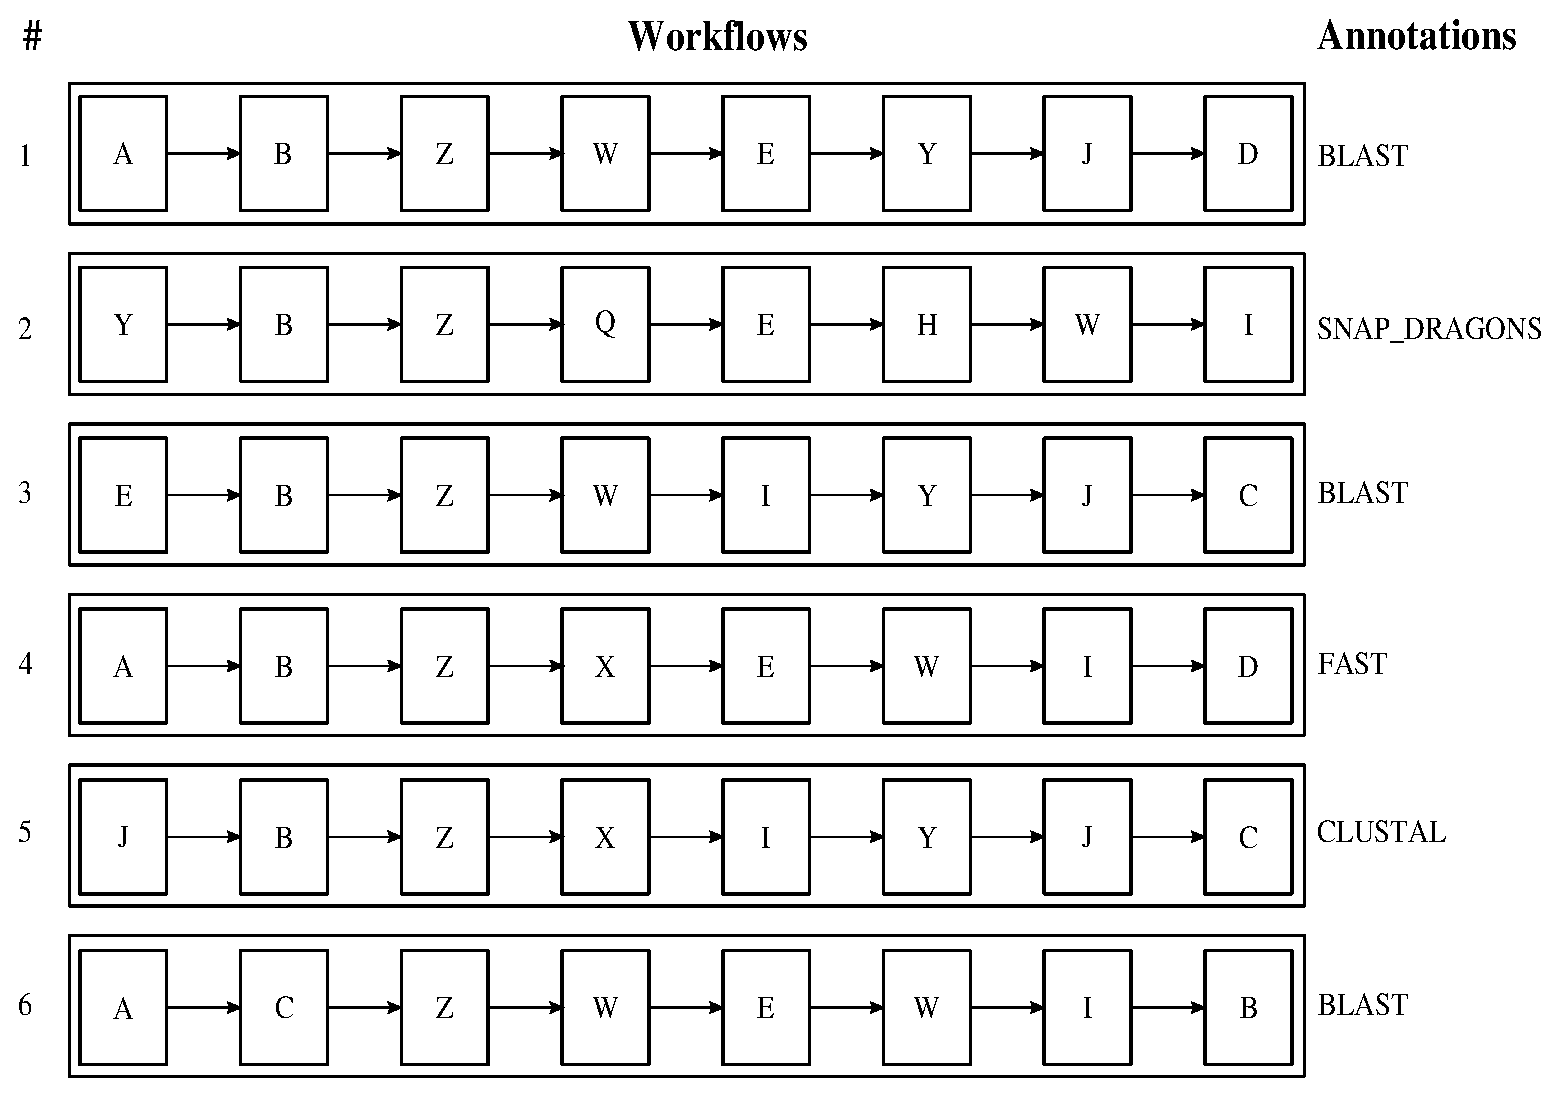
\includegraphics[scale = 0.3]{./pics/recomendacaofreqontologia.eps}
	\caption{{\bf An example of a database of scientific workflows.} Scientific workflows with ontological annotations used to exemplify the proposed solution.}
	\label{FIGURA_ONTOLOGIA_CONSTRUIDA2}
\end{figure}

The FIOO solution begins by calculating the frequency of occurrence of each pair of existing activities, which is the number of times that an activity \emph{W} occurs immediately after another activity \emph{Z}. By considering only activities that have already been connected (on the dataset of workflows), the output and input compatibility is guaranteed.

After calculating the frequency, it is necessary to annotate all the workflows of the figure~\ref{FIGURA_ONTOLOGIA_CONSTRUIDA2}, using the concepts of the domain ontology (see Figure~\ref{FIGURA_ONTOLOGIA_CONSTRUIDA}). This step was performed manually which is a limitation of the work. Finally, the algorithm annotates all activities with the same annotations of their respective workflow; i.e., if the \emph{X} activity (Figure \ref{FIGURA_ONTOLOGIA_CONSTRUIDA2}) is inside two workflows with distinct annotations, then this activity will be related to two different concepts from the ontology. The final result is presented in Table \ref{tabela_lista_recomendacao_ordenada_frequencia}, which contains the activities' frequencies and annotations.

To understand the recommendation training mechanism, another example will be used to simulate a user interacting with the recommendation system. Let us assume that during the construction of the workflow~\(1\) (see Figure~\ref{FIGURA_ONTOLOGIA_CONSTRUIDA}) a scientist inserts the \emph{Z} activity and asks for a recommendation. The system will look at the list of activities that occurs after \emph{Z} sorted by frequency and ontological concept and will return the recommendation list presented in table~\ref{tabela_lista_recomendacao_ordenada_frequencia}. The sorting considering the ontological concepts serves as a tiebreaker criterion when two activities have the same frequency. In this example, according to the recommendation list of Table~\ref{tabela_lista_recomendacao_ordenada_frequencia}, the \emph{W} activity would be first recommended to the user.

\begin{table}[!htb]
	\begin{center}
		\caption{Recommendation for activity \emph{Z} sorted by frequency and ontological concept}
		\label{tabela_lista_recomendacao_ordenada_frequencia}
		%\begin{tabular}{|c|c|c|c|}  \hline
		\begin{tabular}{cccc} \hline
			\textbf{Position} & \textbf{Activ} & \textbf{Frequency} & \textbf{Annotation} 	\\ \hline
			1				& W 				& 3 				& BLAST				\\ 
			2				& X 				& 2 				& FAST, CLUSTAL		\\ 
			3				& Q 				& 1 				& SNAP DRAGONS		\\ 
			\(\vdots\)		& \(\vdots\)		& \(\vdots\) 		& \(\vdots\)		\\ 
			280				& \(\vdots\)		& \(\vdots\)		& \(\vdots\)	\\ \hline
		\end{tabular}
	\end{center}
\end{table}

The activities are annotated with the same annotation of the workflows that contain them. Thus, it is possible that there is at least one activity with more than one annotation. This creates a new recommendation case to consider. Suppose both \emph{W} and \emph{X} activities contains in their annotation lists the concept \emph{BLAST}. In this case, the activity with a lower number of annotations would be recommended, since it is considered more specific for the experiment in question. If both activities have the same number of annotations, the alphabetical order of concepts is used as the tie-breaking criterion. If a new tie occurs a random selector is used.

\subsection{Ontology construction}
The ontology was developed using the Skeletal methodology~\cite{Uschold95} which define the steps: (a) Identify the objective; (b) Capture of ontology; (c) Code; (d) Merge with other ontologies; and (e) Validation.

All these steps were followed in the construction of the ontology. The objective of this ontology was to standardize annotations for workflows and to create an hierarchy to be used in the recommendation step. During the Capture of ontology step, authors studied the bioinformatics area to understand the ontology domain. For the Code step, the Protégé tool\footnote{https://protege.stanford.edu/} was used. No other ontology has found, thus there was no merge step and a domain specialist validated the ontology produced.

\begin{figure}[!htb]
	\centering
	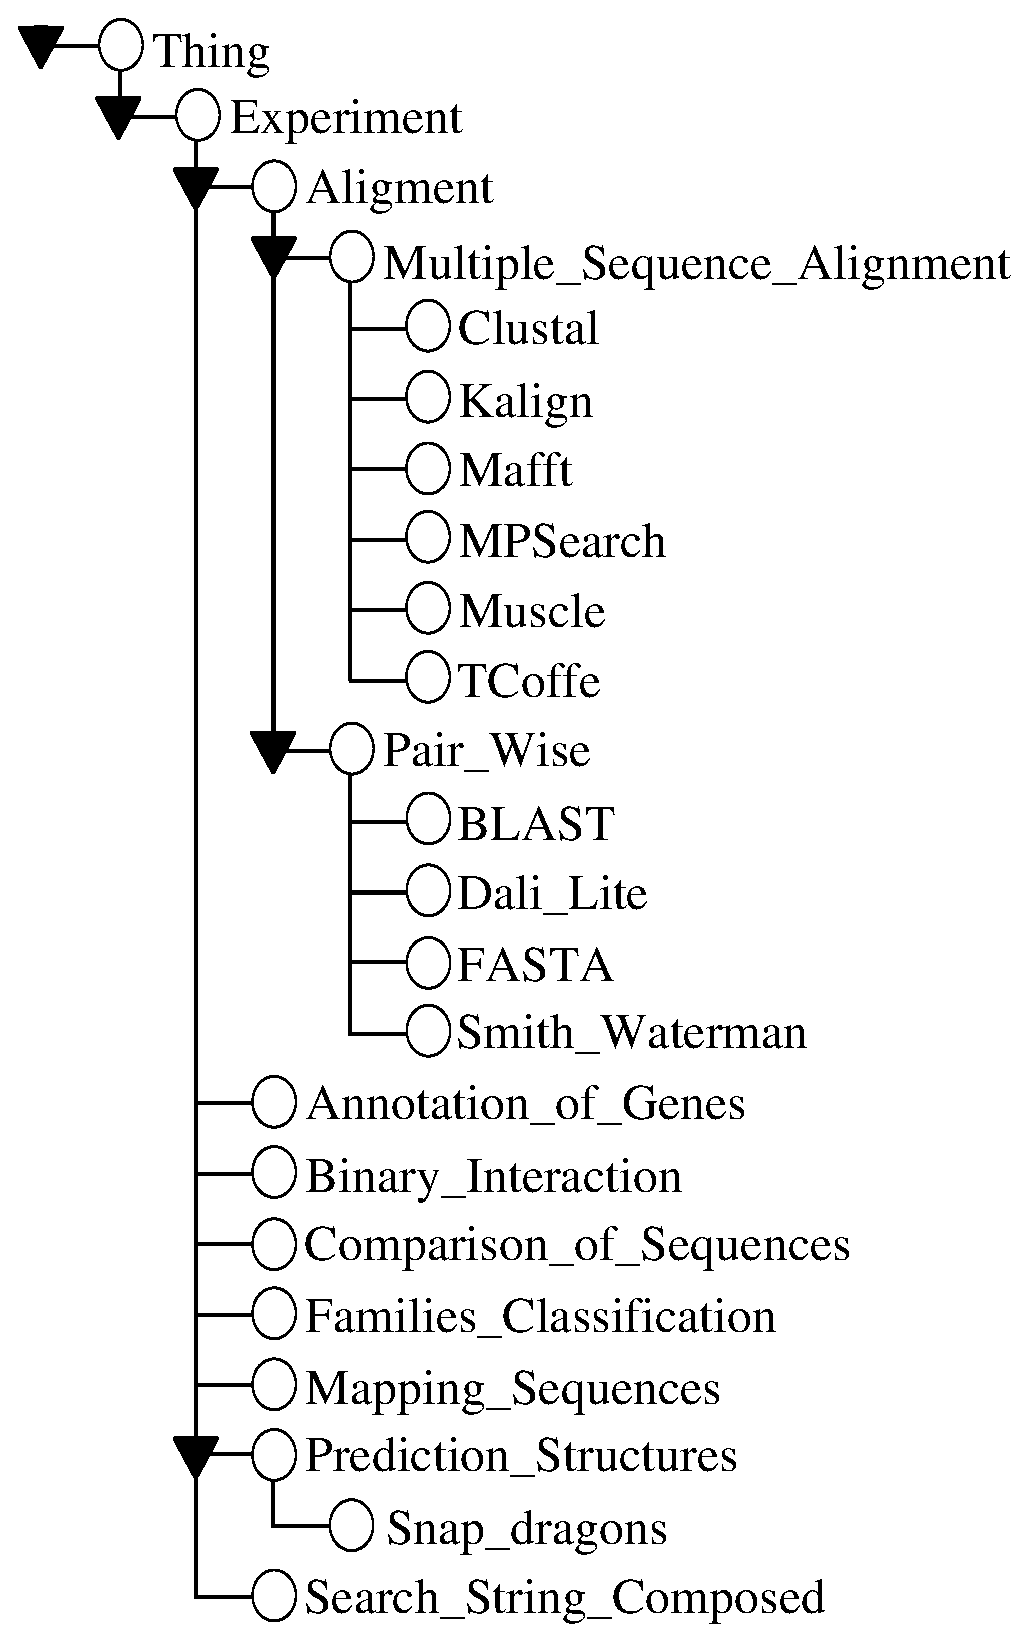
\includegraphics[scale = 0.3]{./pics/ontologia.eps}
	\caption{{\bf Ontology.} Ontology built to annotate scientific workflows with ontological concepts.}
	\label{FIGURA_ONTOLOGIA_CONSTRUIDA}
\end{figure}


\section{Results}
This sections show all the sixteen experiments that were done, each one was a typical machine learning experiment trained by a 10-fold cross validation for each parameter change. Each approach has a typical set of parameters to be optimized during the training step. Table~\ref{tb_parametros} shows all the variations of parameters.
\bgroup
\begin{table}[!htp]
	\begin{center}
		\caption{Recommendation results}
		\label{tb_parametros}
		\begin{tabular}{llllllll} \hline
			\tiny
			\textbf{\(\mathbf{\#}\)} & \textbf{Approach}&\textbf{S@1}&\textbf{S@5} & \textbf{S@50} & \textbf{S@100} & \textbf{S@280} & \textbf{MRR} \\ \hline
			1  & Random					& 0.00 & 0.02 & 0.03 & 0.04 & 1 & 0.033 \\
			2  & \emph{Apriori}			& 0.00 & 0.03 & 0.05 & 0.05 & 1 & 0.037 \\ 
			3  & KNN\(_C\)				& 0.00 & 0.06 & 0.50 & 1.00 & 1 & 0.040 \\ 			
			4  & N. Network\(_C\)		& 0.01 & 0.15 & 0.80 & 1.00 & 1 & 0.089 \\ 
			5  & CART\(_C\)				& 0.02 & 0.12 & 0.76 & 1.00 & 1 & 0.113 \\ 
			6  & CART\(_R\)    			& 0.13 & 0.13 & 0.61 & 1.00 & 1 & 0.114 \\ 
			7  & Naive Bayes\(_C\)     	& 0.02 & 0.15 & 0.63 & 1.00 & 1 & 0.114 \\ 
			8  & Binomial\(_R\) 		& 0.08 & 0.19 & 0.84 & 1.00 & 1 & 0.136 \\ 
			9  & N. Network\(_R\)   	& 0.10 & 0.26 & 0.26 & 1.00 & 1 & 0.154 \\ 
			10 & MARS\(_R\)     		& 0.12 & 0.20 & 0.72 & 1.00 & 1 & 0.167 \\ 
			11 & FIO           			& 0.14 & 0.26 & 0.86 & 1.00 & 1 & 0.196 \\ 
			12 & SVM\(_R\)     			& 0.12 & 0.31 & 0.84 & 1.00 & 1 & 0.238 \\ 
			13 & SVM\(_C\)    			& 0.24 & 0.46 & 0.71 & 1.00 & 1 & 0.244 \\ 
			14 & Comp. SVM\(_C\)		& 0.25 & 0.44 & 0.76 & 1.00 & 1 & 0.314 \\ 
			15 & Rot. Forest\(_C\)  	& 0.29 & 0.45 & 0.77 & 1.00 & 1 & 0.324 \\ 
			16 & FIOO          			& 0.34 & 0.46 & 0.81 & 1.00 & 1 & 0.334 \\ \hline
		\end{tabular}
	\end{center}
\end{table}
\egroup

Table \ref{tb_parametros} displays the results of each recommendation system used. FIOO corresponds to our Frequency Input Output and Ontology approach. The techniques that have the letter \emph{C} in subscript are classifiers; the ones that have letter \emph{R} in subscript are regressors; and those that have nothing are from related literature. Each system makes its recommendations according to its own criteria in an recommendation list. Then the activities not recommended are added to the end of this list. Thus, the correct activity will always be found, and the factor that differentiates the recommendation systems is the position the activities are in the recommendation list, which contains \(280\) positions.

The \emph{Random} approach did not require training. The algorithm only randomly selected activities, forming a list of recommended activities. This system recommended less than \(3\%\) of the correct activities in the top ten positions. Most of the correct activities were rated close to position \(140\) which is the average position of the recommended lists. The metric values \(S@280 = 1\) and \(S@100 = 0.04\) indicate that most of the correct items were found after the hundredth position. This system was used to calculate the simplest baseline.

The system using the \emph{Apriori} technique achieved its best performance when the \emph{confidence} and \emph{support} parameters were defined as \emph{without limitation}, that means, no minimum confidence and support values were defined for the creation of association rules. All rules were considered valid. Even without restricting these values, the results of this technique presented results better than only the \emph{Random} approach. Recommending less than \(6\%\) of correct activities between the \(50\) first positions, its accuracy is still low with the value of \(MRR = 0.037\). The poor results of this technique happened due to the fact the technique disregards the order of the activities during the generation of the rules and, consequently, of the recommendation.

The \emph{KNN}  based approach has been trained considering different values of the parameter \emph{k} (from 1 to 100) which represents the number of nearest neighbours (and using the Euclidean distance as the proximity metric). The best recommendation results for this approach were obtained with \(k = 2\). Even so, less than \(10\%\) of the correct items were found among the top ten items in the list and \(50\%\) of items in the first 50 items. According to the MRR metric, the average position of the recommended items was far from the first position in the list (\(MRR = 0.04\)). These results indicate that classifying activities according to the distance between groups of neighbours is not an appropriate approach to this problem.

The approach which uses an MLP neural network as a classifier had results significantly better than the ones achieved by the \emph{KNN} approach when considering the metric S@1 (\(0.0137\) versus \(0.0037\)). For the training of the network the parameters used were: i) number of neurons \(\eta\) (ranging from \(1:40\)); ii) learning rate \(\alpha\) (ranging from \(10^{-7}: 10\)); iii) two hidden layers; and iv) fully connected architecture. The best classification results were achieved with \(\eta = 18\) and \(\alpha = 10^{-4}\), obtaining \(17\%\) of items ranked among the top ten positions in the list, and \(80\%\) among the \(50\) first positions, which represents an improvement of \(30\%\) when compared with the \emph{KNN} approach. The metric value \(MRR = 0.089\) was twice as high as the one from \emph{KNN}, this growth in precision indicates the neural network generalization power to solve non-linear problems was more efficient than the previous approaches.

The approach which uses CART as a classifier, dealing with categorical data, presented a result superior to the one from neural network. The training used the parameters: i) minimum division value \(\gamma = [0:30]\); ii) maximum final tree size \(\delta = [0:10000]\); iii) minimum variation value to perform a division \(cp = [10^{-7}:10]\); iv) division function (\(\xi\)) as Gini Index or Information Gain. The best result was achieved with \(gamma = 0\), \(\delta = 30\), \(cp = 10^{-3} \), and \(\xi = \) Information Gain.

The results of this approach were approximately twice as good as those of the neural network. This indicates approaches that deal with categorical data by nature has a potential for obtaining good results in problems such the one addressed in this paper. The MRR results were \(26\%\) better than the ones achieved by the MLP based approach, and this approach was able to recommend \(12.3\%\) of the searched items in the first position and 76\% in the first \(50\) positions.

The approach which uses CART as regressor achieve its best results with \(gamma = 2\), \(\delta = 20\), \(cp = 10^{-5}\), and \(\xi = \)Information Gain. The recommendation that used continuous values presented a result superior to \(CART_C\) considering the metrics \(S@1\) and \(S@5\) and worse results for \(S@10\) and \(S@50\). The general precision (MRR) of \(CART_R\) was slightly higher than the one achieved by \(CART_C\).

The Naive Bayes classifier based approach obtained results very similar to the ones achieved by the CART regressor. The training occurred by ranging the \emph{Laplace correction} attribute with values between \([0:100]\). The best result occurred with value zero for this parameter, achieving \(34\%\) of the recommended items in the top ten positions and \(63\%\) among the first \(50\) positions. In contrast, the value of \(MRR\) did not change much.

The binomial regressor approach presented better results when compared with the Naive Bayes and the neural network approaches. The training of this technique occurs using the maximum likelihood for a generalized linear model approximated by a binomial distribution. The results for \(S@5\) and \(S@50\) were higher than the achieved by the previous approaches and the value of the metric \(MRR\) improved by approximately 19\% when compared to the one achieved by the Naive Bayes approach.

The approach which uses a neural network as regressor, considering the weight of the neural network as output, was trained in an analogous way to the neural network used as a classifier. The best result was obtained for the values of \(\eta = 10\) and \(\alpha = 10^{-2}\). It was able to recommend \(26\%\) of the correct items among the top ten positions in the list. System accuracy (MRR) improved \(13\%\) from the achieved by the binomial regressor. These results indicate that using a regressor instead of a classifier presents a better result for this kind of problem, at least when using neural networks.

The approach based on the MARS algorithm as regressor achieved a better result than the one from the neural network (used as regressor). The metric \(S@1\) was improved in \(12.5\%\) and the overall precision (MRR) increased  \(8\%\). This result shows that the curves created by the various connected functions of the MARS obtained a better generalization than the neural network. The training of the parameters was performed using likelihood.

Among the systems proposed in the literature, the system based on input, output and frequency (FIO) (\cite{Wang2008}) is the one with the best results. In the experiments performed, this system identified the correct item among the top ten positions of the recommendation list in \(37\%\) of the cases, and obtained a value of \(MRR = 0.196\).

The SVM regressor presented results twice as good as the MARS algorithm for the metric \(S@10\), since in \(49\%\) of the recommendations the correct item was among the top ten positions in the recommendations list. The MRR value was also higher (\(42\%\)). The training was performed using margin optimization with the values of \(c = [10^{-7}:10^2]\), \(\epsilon = [10^{-7}:10^{2}]\), Tolerance values \(\beta = [10^{-7}:10^{2}]\),  kernel functions: i) linear; ii) sigmoid; iii) polynomial; and (iv) radial. The tested values of the parameter of the polynomial kernel were  \(p = [1:10]\) which is the power of the function. The best results were achieved for \(c = 1\), \(\epsilon = 1\), \(\beta = 10^{-4}\), and polynomial kernel with \(p = 2\). 

The approach based on the SVM algorithm for classification was the only classifier that surpassed the results of the regressors. His training was analogous to the SVM for regression. Its best results were achieved with \(c = 10^{-1}\), \(p = 10^{-4}\), and \emph{linear kernel}. The value of the metric \(S@1\) was \(64\%\) better than the one from FIO technique and the general precision value (MRR) increased \(24\%\). This result indicates that the solution using \emph{kernel} for high-dimensional mapping is an efficient approach in the case of classifiers.

The composed SVM system, which recommends items based on the results of the other recommendation approaches, achieved better results than the SVM. Its training was analogous to that of SVM\(_C\) and its best results were achieved with \(c = 10^{-2}\), \(p = 1\), and polynomial kernel. There was an improvement of \(3\%\) in the metric \(S@1\) and \(28\%\) in the metric \(MRR\), this improvement is due to the use of the result of other classifiers together with the sparsity reduction of the data set.

The system using \emph{Rotation Forest} presented the second best result, its training used the parameters: i) minimum division value \(\gamma = [0:30]\); ii) maximum final tree size \(\delta = [0:10000]\); iii) minimum variation value to perform a division \(cp = [10^{-7}:10]\); iv) division function (\(\xi\)) using Gini Index and Information Gain; v) \(K = [1:10]\) as the number of partitions; vi) \(L = [1:10]\) as the number of classifiers; and (vii) cutoff values \(0.25, 0.5, 0.75\). Is use of an ensemble classification technique was able to achieve better results, for example, \(S@1 = 0.29\), \(S@10 = 0.54\), and \(MRR = 0.324\).

Our ontology-based approach (FIOO) achieved better (or at least equal) results than the previous approaches for almost all of the evaluated metrics. It considers the use of frequency, input, output, and semantic information about the activities. In comparison to the other techniques, its result was higher for all calculated metrics, except \(S@50\) for some techniques. In relation to the FIO technique, its result was superior. In particular, part of this improvement is justified by cases where the correct activity has zero frequency in the training set. Since FIOO considers the ontology information it is able to recommend activities even if they have zero frequency in the train set. In addition, for the case where there is a tie between two activities considering the input, output, and the frequency criteria, the proposed technique presents an additional factor to be used as a tie breaker.

We were able to identify some trends in these results. Increasing information on data in the recommendation improves the recommenders performance, as the result of the experiments: 2, 12, and 14 show. A second trend is that the SVM classifier was the only one that obtained a better result than the regressors, indicating that solutions by maximizing space between data in high dimension may be a promising area of study. A third trend is the use of composite classifiers and\emph{ensembles}, which presented promising results. In the case of the \emph{ensemble}, there is a clue that techniques of this kind, which use thresholds to convert the mean values of the set result \(L\) into binary values, have promising results in recommending activities.

\section{Conclusions}
This work presented a hybrid approach to recommend activities in scientific workflows, called FIOO. It uses syntax compatibility, frequency, and domain ontology to recommend activities. We also modeled the problem of recommendation as an artificial intelligence classification and regression problem. 

Our results were compared with the ones presented in the related literature which was previously identified through a systematic literature review. In this review, we identified techniques, their restrictions, their advantages and the forms that they were validated. 

In order to perform the comparison, a relational database of workflows and their activities was constructed. It was also necessary to establish a methodology to compare different activity recommendation techniques for the same data set with the same validation metrics (\(S@k\) and \(MRR\)).

When comparing all techniques, certain aspects  of  the data set were verified, such as the fact that the activities were not independent; the problem is not linearly separable, and that clustering techniques were not adequate to solve this problem. With the exception  of  SVM, regressors presented more accurate results than classifiers. Finally, adding information in the recommendation systems improved their accuracy.

The extension of this system to another domain is easy. The first step is to develop or find a domain ontology. After that, all the activities should be annotated according to this ontology. Finally, use the recommendation technique described in this paper. If someone does not want to annotate the activities, he/she can use the classification based approaches. In order to do this, it is necessary to only model the workflows as an input for the classifiers, as presented in this paper.

As future work, we intend to investigate the use of data provenance to increase the accuracy of the recommendations. 
Moreover, we will investigate how to automatically annotated the workflows, the main limitation of this paper.

\bibliographystyle{abbrv}
\bibliography{referenciasNovas}

\end{document}